\documentclass[twocolumn,2pt]{jarticle}
\setlength{\columnsep}{3zw} 

\title{画像からユーモアを想起させる説明文章の生成}
\date{}


\usepackage{textcomp}
\usepackage[sc]{mathpazo}
\usepackage[scaled]{helvet}
\usepackage{amsmath,amssymb}
\usepackage{otf}
\usepackage{color}
\usepackage{threeparttable}
\usepackage[dvipdfmx,hiresbb]{graphicx}
\usepackage{float}
\usepackage{fancyhdr}
\usepackage{titlesec}
\usepackage[top=30truemm,bottom=30truemm,left=25truemm,right=25truemm]{geometry}

%define for header
\titleformat*{\section}{\large\bfseries}
\renewcommand{\ttdefault}

%Header
\pagestyle{fancy}
\lhead{}
\rhead{出願研究科: 情報科学研究科\\希望希望研究室: 知能コミュニケーション研究室 \\ 氏名: 二又航介}

\begin{document}
\small
\maketitle

\section{はじめに}
\thispagestyle{fancy}

私が,奈良先端科学技術大学院大学(以下NAIST)で取り組みたい研究テーマは「画像からユーモアを想起させる文章の生成」である.本稿では,この研究テーマの研究背景及び目的,先行研究,そして提案手法について述べる.

\section{研究の背景,目的}
近年AppleのSiriやSoftbankのPepperなど,ヒトと対話的なインタラクションを行う対話システムが数多く提案されている.
日常生活で用いられるシステムやエンターテイメント性が要求されるシステムではユーザーを飽きさせない,対話継続欲求の高いデザインを採用する必要がある.
宮澤らは人同士のインタラクションを参考に,毎回の対話において「次回も続けたい」と感じる要因を分析することで,対話継続欲求の高いシステムのデザイン方法の確立を目指してきた\cite{宮澤}.
分析の結果,「対話において相手の発話行動を限定しないこと」,「相手の話を聞いている実感を与えること」,「人工物であることを生かした意外性の高いユーモアを使うこと」が有効であることが明らかになった.



以上の知見を参考に,藤倉らはユーモア応答を用いることでユーザーの対話継続欲求の向上を目指した\cite{藤倉}.
しかし,ユーザーの言語情報に基づきユーモア発話を生成する試みは,ユーザーが発話を辞めた時点で閉ざされてしまう.
ユーモアは言語情報のみならず,視覚情報などからも生成可能である.
例えば,友人が誰かのモノマネをしている時に,「ツッコミ」を入れる場面が考えられる.
視覚情報を下にユーモア発話を生成すれば,ユーザーの言語情報に限定されないユーモアが生成可能であると想定される.
さらに視覚情報を用いてシステムがユーモアを自ずから生成することができれば,ユーザーが発話を行う必要がないため,ユーザーがシステムの利用をやめてしまってもユーモア生成の可能性が閉ざされない.
システムによって生成されたユーモアに対して,ユーザーが面白さを感じることができれば,システムが再利用される可能性が残されるだろう.
そこで本研究では,画像からユーモアを想起させる文章を生成することで,ユーザーの対話継続欲求を向上させることを目指す.
図\ref{fig:conf}に,システムがユーモア文章を生成する流れを示す.
初めに,システムがユーザーなどの写真を撮影する.
次にシステムが,撮影した画像から「立派なサボテンが微笑んでいますね!」などのユーモア文章を生成し,音声,またはテキストデータとしてユーザーに提示する.
最後に,ユーザーが提示されたユーモアを受容する.
ユーザーがユーモアを受容した際,面白さを感じることができれば,ユーザーの対話継続欲求が高まると想定される.




\begin{figure}
	\begin{center}
		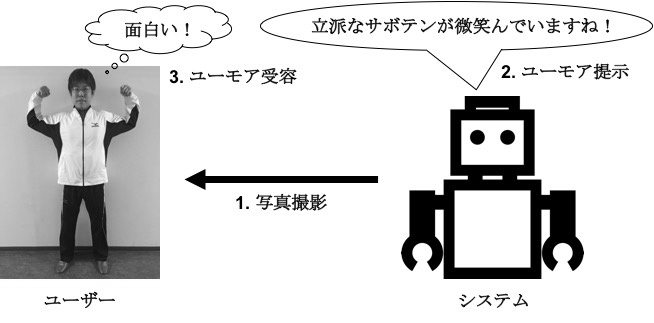
\includegraphics[width=7cm]{images/abstract_gray.jpg}
		\caption{システムによるユーモア文章生成の流れ}
		\label{fig:conf}
	\end{center}
\end{figure}


\section{先行研究}
ユーモアに関わる認知的メカニズムを説明する理論として「不適合理論\cite{incongruity}」がある.
%考えるモデル > するモデル
「不適合理論」には,ユーモアの生成因を不適合そのものに求める「不適合モデル\cite{incongruity}」や,その解決に求める「不適合-解決モデル\cite{resolution}」がある.
「不適合モデル」は,期待の心象と実際の刺激が異なることにより発生する不適合そのものによってユーモアが引き起こされると考えるモデルである.
例えば,一発芸やナンセンスなジョークなどが「不適合モデル」に対して当てはまりが良いとされる.
一方,「不適合-解決モデル」は,不適合に対して論理的な脈絡を発見することにより解決の過程が導かれ,その結果ユーモアが引き起こされると考えるモデルである.
例えば,漫才の「ボケ」に対する「ツッコミ」はボケが生じさせた不適合を解決する手がかりを与える役割を持っている.
「不適合-解決モデル」は解決という概念の導入により,不適合モデルに比べ,多くのユーモア現象を説明できる\cite{統合モデル}.
また,曖昧さ耐性の低い個人ほど,「不適合モデル」より「不適合-解決モデル」を好むという結果が明らかになっている\cite{Ruch}.


ユーモア現象は,単語間類似度の観点からも説明できる.
Kaoらは,AmbiguityとDistinctivenessの観点から駄洒落の面白さを説明しており,実験の結果から置換される対象の単語と置換後の単語が同じ文脈で発生しやすく,かつ置換される単語と置換後の単語間の関連性が小さいほどユーモアの受容性が向上すると示した\cite{kao}.
従って,単語間の類似度は不適合の強さを表していると想定される.


\section{提案手法}
前節で述べたように,「不適合-解決モデル」は「不適合モデル」と比較すると、より多くのユーモア現象を説明することができ,かつより多くの人にユーモアとして受容されると想定される.
そこで,本研究では,「不適合-解決モデル」に基づき,画像からユーモア文章を生成することを目指す.
単語間の類似度は不適合の強さを表していると想定されるため\cite{kao},生成されるユーモア文章における単語と画像に写る対象を表す単語の関連度が小さいほどユーモアの受容性が向上すると想定される.
しかし,単語間の類似度を考慮するだけでは,解決の過程が導かれないため,「不適合-解決モデル」を当てはめたユーモアとして受容されないだろう.
そこで,画像間類似度を計算することで解決の過程を導く.
画像に写る対象と生成される文章における単語を表す画像の画像間類似度が高ければ,両者が類似しているという観点から解決の過程が導かれると想定される.
つまり,生成される単語と画像に写る物体の単語間類似度が低いことにより不適合が生じ,それらの画像間類似度が高いことにより解決の過程が導かれる.



本研究において提案する類似度計算の過程を図\ref{fig:flow}に示す.
初めに,画像を入力し,システムによって予め用意されたオブジェクトデータと画像間類似度を比較し,入力画像に写る物体と類似する物体を選択する.
オブジェクトデータは,「イヌ」,「カンガルー」,「カカシ」,「サボテン」など様々な物体の画像と,その画像に対応する名詞のペアから構成される.
画像間類似度が高いほど,解決の過程が容易になると想定されるため,入力画像とオブジェクトデータを比較した際,画像間類似度が高いと想定される「カカシ」、「サボテン」を選択する.
次に,単語間類似度を計算する.
単語間類似度が低いほど,不適合が強まると想定されるため,画像間類似度の計算過程で洗濯された「カカシ」,「サボテン」のうち,入力画像を表す名詞である「人間」との単語間類似度が低いと想定される「サボテン」を最終的に選択する.



画像間類似度を計算方法として,CNN(Convolutional Neural Network)を用いる.
CNNは分類タスク用に学習済みのモデルを利用し,最終層手前のFeed Forward層から取得される特徴ベクトルを用いて$cos$類似度によって類似度計算を行う.
単語間類似度の計算方法についても,画像間類似度の計算と同様に,単語を特徴ベクトルに変換し,cos類似度を用いることによって類似度計算を行う.


%姿勢データを`特徴`として記述
%画像の特徴としてこのような感じだと理解できる


\begin{figure}
	\begin{center}
		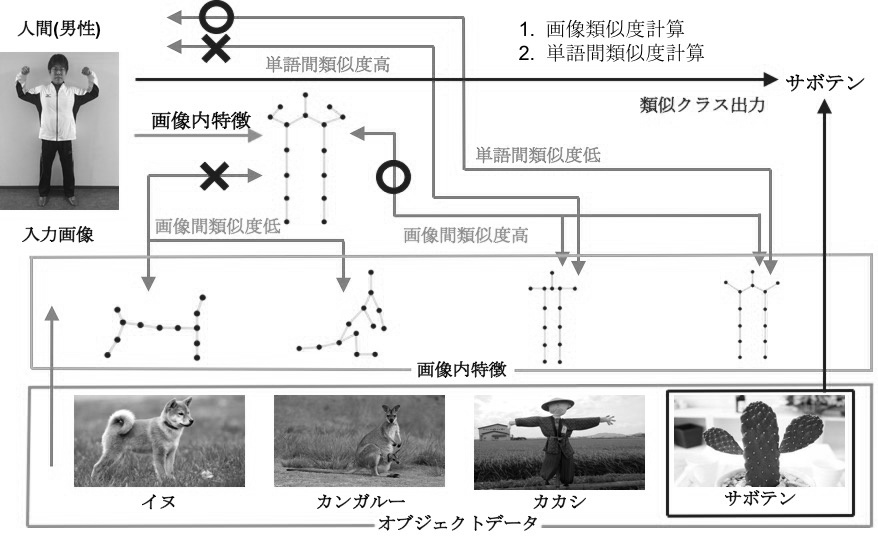
\includegraphics[width=7cm]{images/flow_gray.jpg}
		\caption{類似度計算の過程}
		\label{fig:flow}
	\end{center}
\end{figure}



上述の手法を用いて文章内の単語を他のオブジェクトと置換することで,文章がユーモアとして受容されると想定される.
提案手法では,Neural Image Caption(NIC)\cite{NIC}を用いて,上述の手法を取り入れたモデルの構築を目指す.
NICとは,画像に写る状況を説明文章を生成する手法である.
NICにより生成された文章の主語と類似度計算により導出された単語を置換した結果を,ユーモア文章として扱う.
NICにより生成された文章に対して,単語の置換を行うことで,画像と文章のミスマッチにより,より不適合が強まると想定される.


%本研究で扱うユーモアは「テキスト刺激によって不適合が生じ,画像とテキストから解決が導かれ,かつ刺激の受容者が面白いと感じるもの」として定義する.


%CNN>LSTMの流れ
%技術的なことをもっとかく
%考えられる > 想定される、懸念される
%なになに的はだめ



%初めに入力として画像を受け取り,その画像に基づきキャプションを生成する.
%生成されたキャプションから,主語を抽出し,その主語と一致する物体を検出する.
%物体検出の結果とシステムによって予め準備されたオブジェクトデータとの画像間類似度を比較し,画像間類似度が大きいオブジェクトを取得する.
%次に,キャプションから抽出された主語と画像間類似度が大きいオブジェクトの単語間類似度を計算し,単語間類似度が小さいオブジェクトを取得する.
%最後に,画像間類似度が大きく,単語間類似度が小さいオブジェクトを,生成されたキャプションの主語と置き換えた結果をユーモア文章として用いる.


\section{まとめ}
本稿では,私がNAISTで取り組みたい研究テーマである「画像データからユーモアを想起させる説明文章の生成」の研究概要について述べた.
研究の流れとしては初めに,本研究で提案するユーモア文章の生成手法の検証及び必要に応じて改良を行う.
次に,提案手法に基づき,システムを設計,開発する.
最後に,システムによって生成されたユーモア文章がユーザーにユーモアとして受容されるかどうか検討するため,ユーモア評価実験を行い,実験結果からシステムの妥当性を検証する.
%最後に作成したシステムを用いてユーモア評価実験を行い,実験結果からシステムの妥当性を検証する.
本研究では,画像間類似度が大きく、単語間類似度が小さい単語を文章内に用いることで,ユーモアとして受容されると想定している.
従って,ユーモア評価実験において,画像間類似度及び単語間類似度の変化によってユーモアの受容性がどのように変化するか検討する.


\bibliographystyle{jplain}
\bibliography{Untitled}

\end{document}